\renewcommand{\thispart}{1 }
\renewcommand{\thispartname}{Introduction to Machine Learning}

\part{\thispartname}

% Cover page
%
% Cover page for giveb part
%

\title[\modulename - Part \thispart]
{
  {\bf 
   \modulename - 
   Part \thispart\\
  }
  \vspace{0.5cm}
  {\it 
   \color{yellow}
    \secname\\
  }
}
\author[C.Andreopoulos] {
  Professor Costas Andreopoulos\inst{1,2}, {\it FHEA}
}
\institute[Liverpool/STFC-RAL] {
   \inst{1} University of Liverpool, Department of Physics\\
   \vspace{0.3cm}
   {\it {\color{magenta} Lectures delivered at the University of Liverpool, 2024-25}}\\
   \vspace{0.2cm}
}
\date{\today}

\titlegraphic{
  
\includegraphics[height=30px]{images/logo/liverpool.png}
}

\begin{frame}[plain]
  \titlepage
\end{frame}




% Outline
\section{Outline}
%
% Table of contents to be displayed at the beginning of each part
%

\begin{frame}[t,allowframebreaks]{Outline for Part \thispart -}
  % Part \thispart (\secname) covers the following topics:\\
  % \vspace{0.5cm}
  \linespread{1.1}
  \setcounter{secnumdepth}{3}
  \setcounter{tocdepth}{3}
  % \tableofcontents[currentsection, hideothersubsections, sectionstyle=hide/hide]
  \tableofcontents[part=\thispart]
\end{frame}



% AI
\section{Artificial intelligence}
\begin{frame}{Artificial Intelligence}

    \index{artificial intelligence}\index{AI}\gls{ai} 
    can be defined as the 
    `{\bf science and engineering of making intelligent 
    machines}' \cite{McCarthy:2007ai}.\\
    \vspace{0.2cm}
    Intelligence: 
    \begin{itemize}
        \item can be difficult to define \cite{Neisser:1996intl},
        \item is an umbrella term for several skills and abilities, and
        \item is generally understood in relation to human intelligence \cite{McCarthy:2007ai}.\\
    \end{itemize}
    \vspace{0.1cm}
    \begin{block}{}
    Generally, intelligence is the capacity to {\bf acquire information}, 
    {\bf convert it to knowledge}, and {\bf apply that knowledge} 
    to think abstractly or while interacting with the environment.\\
    \end{block}
    \vspace{0.1cm}
    There are many types of intelligence.\\
    \vspace{0.1cm}
    Humans, animals, and some machines display varying levels of intelligence.\\
    
\end{frame}
    

% Precursors of AI
\section{Precursors of artificial intelligence}
%
%
%

\begin{frame}[t, allowframebreaks]{Precursors of Artifial Intelligence -}

    \vspace{-0.1cm}
    We always dreamt of {\bf building machines with human-like intelligence}!\\
    \begin{itemize}
        \small
        \item
        Master craftsmen and intelligent machines in many myths and stories.\\
    \end{itemize}
    \vspace{-0.4cm}

    \begin{columns}[t]
        \begin{column}{0.46\textwidth}
         \begin{center}
          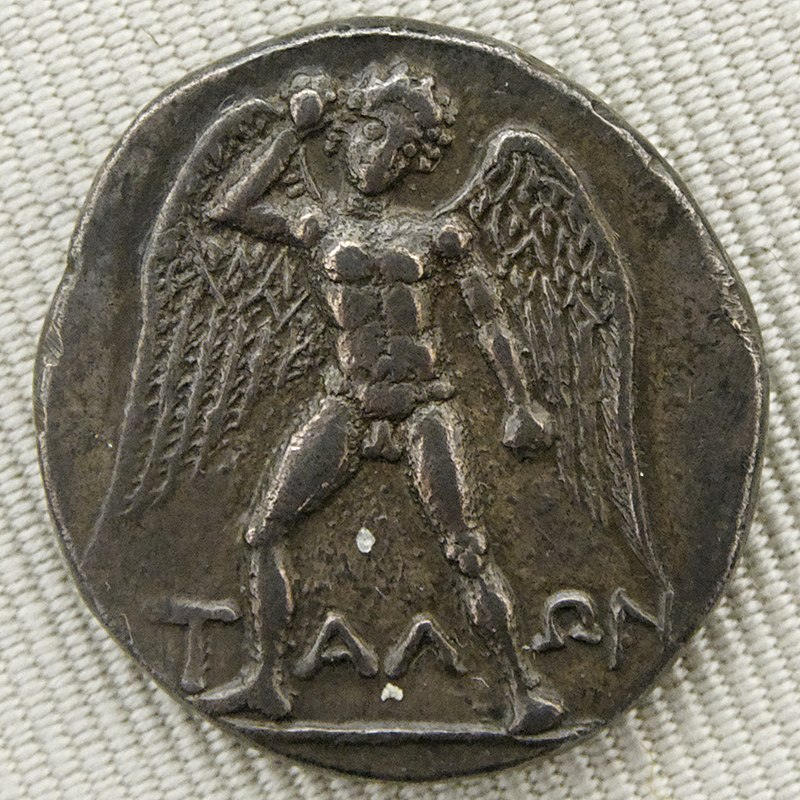
\includegraphics[width=0.99\textwidth]{./images/precursors/talos.jpg}\\
          {\scriptsize 
          \vspace{0.1cm}
          Talos on a Greek coin from 300 BCE.\\
          \color{col:attribution} 
          (Cabinet des Médailles, Paris.)
          \href{https://en.wikipedia.org/wiki/Talos\#/media/File:Didrachm_Phaistos_obverse_CdM.jpg}{\tiny [link]}
          \\}
         \end{center}
        \end{column}
        \begin{column}{0.54\textwidth}
            \begin{itemize}
                \small
                \item 
                {\bf Talos}, the bronze giant built by the god
                Hephaestus to protect Crete from invaders.
                \href{https://en.wikipedia.org/wiki/Talos}{\tiny [Wikipedia]}
                \item 
                {\bf Galatea}, the female ivory statue animated 
                by the goddess Aphrodite when its sculptor, Pygmalion, 
                fell in love with it.
                \href{https://en.wikipedia.org/wiki/Pygmalion_(mythology)}{\tiny [Wikipedia]}
                \item
                {\bf Golems} in Jewish folklore, made from clay 
                and animated by words written on their foreheads, 
                or on pieces of paper placed in their mouth.
                \href{https://en.wikipedia.org/wiki/Golem}{\tiny [Wikipedia]}
                \item
                {\bf Homunculi} (sing.: Homunculus), 
                the little anthropomorphic creatures found in alchemical traditions.
                \href{https://en.wikipedia.org/wiki/Homunculus}{\tiny [Wikipedia]}
            \end{itemize}        
        \end{column}
    \end{columns}

    \framebreak

    \begin{itemize}
        \small
        \item
        {\bf Brazen heads}, the future-telling automata of 
        Gerbert of Aurillac, Saint Albertus, Robert Grosseteste, 
        and Roger Bacon.
        \href{https://en.wikipedia.org/wiki/Brazen_head}{\tiny [Wikipedia]}\\
        \item
        {\bf Frankenstein!} by Marry Shelley (1818).
        
\includegraphics[width=0.04\textwidth]{./images/precursors/stein.jpg}
        \href{https://en.wikipedia.org/wiki/Frankenstein}{\tiny [Wikipedia]}\\
        \item
        {\bf Hadaly}, the female android in the science fiction novel `The Future Eve' (1886)
        by Auguste Villiers de I'Isle-Adam.
        \href{https://en.wikipedia.org/wiki/The_Future_Eve}{\tiny [Wikipedia]}\\
        \item
        {\bf Maria} in the science fiction movie `Metropolis' (1927)
        \href{https://en.wikipedia.org/wiki/Metropolis_(1927_film)}{\tiny [Wikipedia]}\\
    \end{itemize}        

    \vspace{-0.3cm}

    \begin{columns}[t]
        \begin{column}{0.32\textwidth}
            \begin{center}
                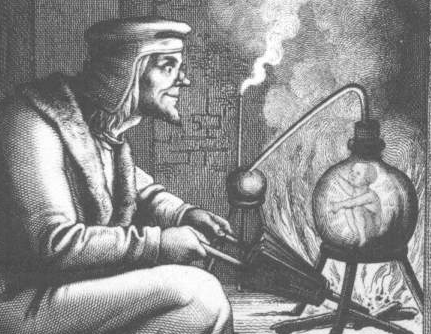
\includegraphics[width=0.99\textwidth]
                {./images/precursors/homunculus_cropped.png}\\
                {\scriptsize 
                \vspace{0.1cm}
                19$^{th}$ century engraving of Wagner and Homunculus 
                from Goethe's Faust II.
                \href{https://en.wikipedia.org/wiki/Homunculus\#/media/File:Faust_image_19thcentury.jpg}{\tiny [link]}\\
                }
            \end{center}
        \end{column}
        \begin{column}{0.37\textwidth}
            \begin{center}
                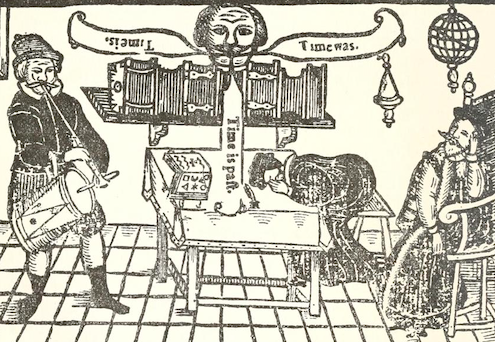
\includegraphics[width=0.99\textwidth]
                {./images/precursors/brazen_head_cropped.png}\\
                {\scriptsize 
                \vspace{0.1cm}
                Reprint of 1630 edition of 
                Robert Greene's Friar Bacon and Friar Bungay.
                \href{https://en.wikipedia.org/wiki/Friar_Bacon_and_Friar_Bungay\#/media/File:Greene_Bacon_and_Bungay_1630.jpg}{\tiny [link]}\\
                }
            \end{center}
        \end{column}
        \begin{column}{0.30\textwidth}
            \begin{center}
                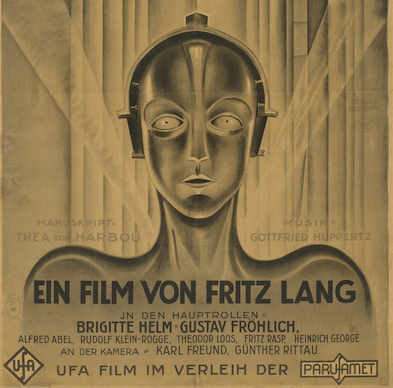
\includegraphics[width=0.80\textwidth]
                {./images/precursors/metropolis_cropped.png}\\
                {\scriptsize 
                \vspace{0.1cm}
                Part of the theatrical release poster for Metropolis,
                by Heinz Schulz-Neudamn.
                \href{https://en.wikipedia.org/wiki/Metropolis_(1927_film)\#/media/File:Metropolis_(German_three-sheet_poster).jpg}{\tiny [link]}\\
                }      
            \end{center}
        \end{column}
    \end{columns}

\end{frame}

% Types of AI
\section{Types of artificial intelligence}

%
%
%

\begin{frame}{Types of Artifical Intelligence}

    Classification based on capabilities (Type-1):\\
    \vspace{0.1cm}

    \begin{itemize}

        \item 
        \index{artificial narrow intelligence}\index{ANI}
        \gls{ani}, often referred to as 
        \index{weak AI}\Gls{weak ai} or
        \index{narrow AI}\Gls{narrow ai}:
        This is \index{artificial intelligence}\index{AI}\gls{ai} 
        with a {\bf narrow range of capabilities}.\\

        \vspace{0.1cm}

        \begin{itemize}
            \item 
            Only type of \gls{ai} that is {\bf successfully implemented to date}
            \item
            Examples: 
            self-driven cars, voice assistants, 
            face recognition tools, spam filters,
            news feed personalization in social media, 
            chatbots etc.
            \item 
            Trained for specific tasks in a {\bf narrow domain}.   
            \item 
            {\bf Imitates intelligence}, rather than being intelligent.\\
        \end{itemize}

        \vspace{0.1cm}

        \item 
        \index{artificial general intelligence}\index{AGI}
        \gls{agi}, often referred to as 
        \index{strong AI}\Gls{strong ai} or
        \index{deep AI}\Gls{deep ai}:
        \gls{ai} with {\bf human-level capabilities}.\\

        \vspace{0.1cm}

        \begin{itemize}
            \item 
            {\bf Autonomous systems} that {\bf can learn any task}.
            \item 
            Currently, there is no such system.
            \item
            72 \index{agi} R\&D projects were identified as being active in 2020 \cite{GCRI:2020agi}.
        \end{itemize}


        \vspace{0.1cm}
        \item 
        \index{artificial superintelligence}\index{ASI} 
        \gls{asi}:
        \gls{ai} that greatly {\bf exceeds human capabilities} - A hypothetical concept.

    \end{itemize}
    
\end{frame}

%

\begin{frame}{Types of Artifical Intelligence}

    Classification based on functionality (Type-2):\\

    \begin{itemize}

        \item 
        \index{reactive AI}\index{artificial intelligence}\index{AI}\Gls{reactive ai}
        \begin{itemize}
            \item 
            Task-specific \gls{ai} that reacts to inputs and is 
            predictable (it always produces a given response for a given set of inputs)
            \item 
            Does not store memories and does not learn from experience.
            \item
            Example: IBM's Deep Blue chess-playing \gls{ai} system
        \end{itemize}

        \item 
        \index{limited memory AI}\Gls{limited memory ai}
        \begin{itemize}
            \item 
            Task-specific \gls{ai} that stores memories (for a limited time period) 
            and learns from its experiences.
            \item
            Example: Self-driven cars
        \end{itemize}

        \item 
        \index{theory of mind AI}\Gls{theory of mind ai}
        \begin{itemize}
            \item 
            Next-level \gls{ai} system, able to learn any task and exhibit common sense.
            \item 
            Emotionally intelligent, would be able to interact with human emotions
            and adjust its behaviour, show empathy, and understand moral norms.
        \end{itemize}

        \item 
        \index{self-awareness AI}\Gls{self-awareness ai}
        \begin{itemize}
            \item Would attribute mental states not only to others, but also to self.
            \item \gls{ai} with human-level artificial consciousness.
        \end{itemize}

    \end{itemize}
    
\end{frame}


% Human vs computer intelligence
\section{Human vs computer learning}
%
%
%

\begin{frame}[t]{Intelligence?} 

    Imitating intelligence, let alone achieving genuine 
    intelligence, is very hard!\\
    \vspace{0.2cm}

    \begin{columns}
        \begin{column}{0.27\textwidth}
         {\small
           A small sample of \index{AI}\gls{ai} failures that hit the 
           news recently are listed on the right.\\
         }   
         \begin{center}
          
\includegraphics[width=0.98\textwidth]{./images/misc/malfunctioning_robot_1.png}\\
         \end{center}
        \end{column}
        \begin{column}{0.73\textwidth}        
            \begin{itemize}
                \small
                \item 
                Teslas running Autopilot involved in 273 crashes reported in 2021-22.
                \href{https://www.washingtonpost.com/technology/2022/06/15/tesla-autopilot-crashes/}
                {\small [$\rightarrow$ Washington Post article]}
                \item 
                False facial recognition match leads to Black man’s arrest.                
                \href{https://edition.cnn.com/2021/04/29/tech/nijeer-parks-facial-recognition-police-arrest/index.html}
                {\small [$\rightarrow$ CNN article]}
                \item 
                OpenAI GPT-3 medical chatbot designed to help doctors manage 
                their daily workload, told a mock patient to kill themselves.
                \href{https://www.theregister.com/2020/10/28/gpt3_medical_chatbot_experiment/}
                {\small [$\rightarrow$ The Register article]}
                \item 
                A beauty contest was judged by AI and the robots didn't like dark skin.
                \href{https://www.theguardian.com/technology/2016/sep/08/artificial-intelligence-beauty-contest-doesnt-like-black-people}
                {\small [$\rightarrow$ The Guardian article]}
                \item 
                New Zealand passport robot tells applicant of Asian descent to open eyes.
                \href{https://www.reuters.com/article/us-newzealand-passport-error-idUSKBN13W0RL}
                {\small [$\rightarrow$ Reuters article]}
                \item 
                Tay, Microsoft's pro-nazi anti-feminist AI chatbot.\\
                \href{https://www.theguardian.com/technology/2016/mar/24/tay-microsofts-ai-chatbot-gets-a-crash-course-in-racism-from-twitter}
                {\small [$\rightarrow$ The Guardian article]}
            \end{itemize}

        \end{column}
    \end{columns}

    \vspace{0.2cm}
    {\small
      A large list of hilarious failures, mainly from gaming \gls{ai}, 
      is maintained at \cite{GoogDoc:GamingExamplesinAI}.
    }

\end{frame}

% \begin{itemize}
%     \small
%     \item 
%     Neural nets evolved to classify edible and poisonous 
%     mushrooms took advantage of the data being presented 
%     in alternating order, and didn't actually learn any 
%     features of the input images \cite{Lehman:2019Surprising}
%     \item 
%     PlayFun algorithm deliberately dies in the Bubble Bobble 
%     game as a way to teleport to the respawn location
%     \item 
%     Creatures bred for speed grow really tall and 
%     generate high velocities by falling over
%     \item 
%     In an artificial life simulation where survival required 
%     energy but giving birth had no energy cost, one species 
%     evolved a sedentary lifestyle that consisted mostly of 
%     mating in order to produce new children which could be 
%     eaten (or used as mates to produce more edible children).
%     \item 
%     Agent kills itself at the end of level 1 to avoid losing in level 2
%     \item 
%     In a football game, the player is supposed to try 
%     to score a goal against the goalie, one-on-one. 
%     Instead, the player kicks it out of bounds. 
%     Someone from the other team has to throw the 
%     ball in (in this case the goalie), so now the player has a clear shot at the goal.
%     \item 
%     Rewarding a football robot for touching the ball 
%     caused it to learn to get to the ball and vibrate 
%     touching it as fast as possible
%     \item 
%     CycleGAN algorithm for converting aerial photographs 
%     into street maps and back, trained to minimise the cyclic 
%     consistency loss, encoded output information in the intermediary 
%     image without it being humanly detectable.
% \end{itemize}        

%
%
%


\begin{frame}[t,allowframebreaks]{Human vs computer intelligence -} 

\begin{itemize}
\item Computers can 
\end{itemize}

\end{frame}

% History of AI
\section{History of artificial intelligence}
\begin{frame}{The history of AI\footnote{
\tiny For a detailed discussion, see \url{https://en.wikipedia.org/wiki/History_of_artificial_intelligence}}}

\begin{itemize}
\item Birth of AI (1952-1956)
\item Symbolic AI (1956-1974)
\item First AI winter (1974-1980)
\item Boom (1980-1987)
\item Bust: Second AI winter (1987-1993)
\item AI (1993-2011)
\item Deep learning, big data and AI (2011-present)

\end{itemize}

\end{frame}


\subsection{Birth of AI (1952-1956)}
%
%
%

\begin{frame}[t]{Birth of AI (1952-1956)} 

    Several developments in the first half of the 20th century:
    \begin{itemize}
        \item Discovery that the {\bf brain is an electrical network of neurons}
        \begin{itemize}
            \item 
              Richard Caton reported to British Medical Association 
              the first observation of electrical impulses from the 
              brains of living animals (1875) \cite{Caton:1875}.
            \item 
              Hans Berger recorded the first human 
              electroencephalogram (1924) \cite{Berger:1929}.
        \end{itemize}
        \item 
        Development of {\bf control and communication theory} (cyberneutics) 
        \begin{itemize}
            \item by Norbert Wiener
        \end{itemize}
        \item 
        Development of {\bf information theory} 
        \href{https://en.wikipedia.org/wiki/Information_theory}{\tiny [Wikipedia]}
        \begin{itemize}
            \item Early work by Harry Nyquist and Ralph Hartley in 1920's.
            \item Foundations established by Claude Shannon in the 1940's \cite{Shannon:1948}.
        \end{itemize}
        \item 
        Development of {\bf theory of computation} 
        \href{https://en.wikipedia.org/wiki/Theory_of_computation}{\tiny [Wikipedia]}
        \begin{itemize}
            \item John von Neumann, Alan Turing, Alonzo Church and others
        \end{itemize}
    \end{itemize}
    \vspace{0.2cm}
    In early 1950's it became possible to {\bf start imagining a digital brain}!
            
\end{frame}
    
    
    
%
%
%

\begin{frame}[t]{Turing's `Computing Machinery and Intelligence' (1950)} 

    Landmark paper by \gls{Turing}\cite{Turing:1950tt} - Possibility of creating machines that think
    Turing test

\end{frame}

\begin{frame}[t]{SNARC (1951)} 

A first neural net machine, \gls{snarc}, 
was built by \gls{Minsky} and \gls{Edmonds} in 1951.

\begin{columns}
    \begin{column}{0.45\textwidth}
      They design of \gls{snarc} drew inspiration from the work of 
      \gls{McCulloch} and \gls{Pitts} on
      artificial neurons.           
     \begin{center}
        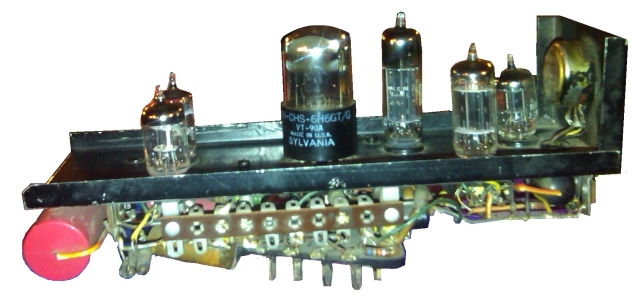
\includegraphics[width=0.99\textwidth]
        {./images/snarc/gregoryloan_snarc_hebbsynapse.png}\\
     {\scriptsize 
      A photograph by Gregory Loan of the only surviving \gls{snarc} neuron.\\
      \color{col:attribution} 
      Photo reproduced from \cite{CyberneticZoo:1951MazeSolver}}\\
     \end{center}
    \end{column}
    \begin{column}{0.55\textwidth}
       \begin{itemize} 
        \item
        \gls{snarc} was a randomly connected network 
        of about 40 neurons (Hebb synapses).
        \item
        Each neuron had a short-term memory and a long-term memory.
        \item
        The machine was trained by navigating a virtual maze 
        (i.e. \gls{snarc} was a "mechanical rat").
        \item
        Actions resulting to a positive reward (provided manually 
        by an operator), engaged a chain that turned a potentiometer 
        (whose setting was analogous to a weight in modern digital networks).
       \end{itemize}
    \end{column}
\end{columns}

\end{frame}
%
%
%

\begin{frame}[t]{Logic Theorist} 

Logic Theorist was a computer program that could perform 
some level of automated reasoning. \cite{Newell:1956logth}
    
\end{frame}
%
%
%

\begin{frame}[t,allowframebreaks]{Dartmouth conference (1956) -} 

    \vspace{-0.2cm}

    \begin{columns}
        \begin{column}{0.62\textwidth}
            \begin{center}
            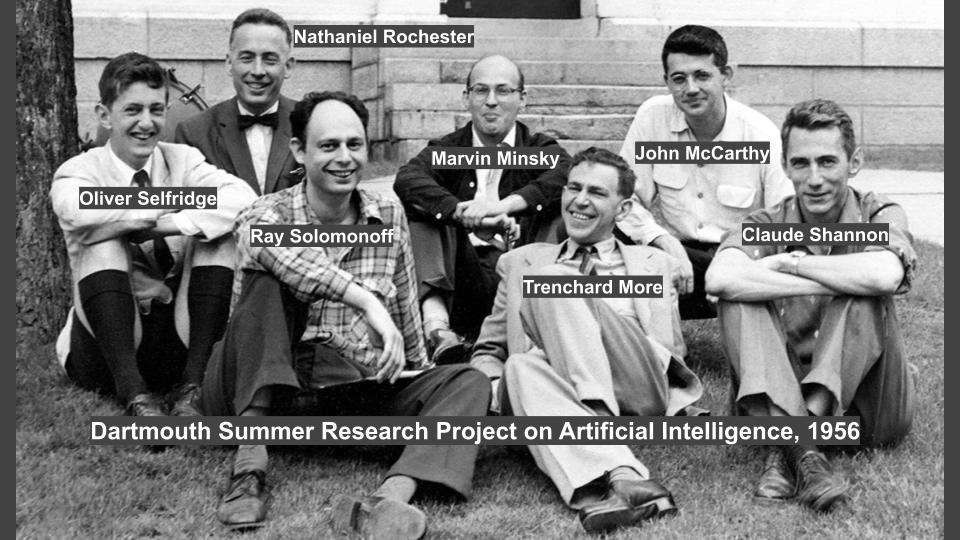
\includegraphics[width=0.98\textwidth]{./images/people/dartmouth_1956.jpg}\\
            { \scriptsize 
            \vspace{0.1cm}
            Participants in the Dartmouth Summer Research Project 
            on Artificial Intelligence, 1956.\\
            \color{col:attribution} 
            Photo labelled by Mindy McAdams
            \href{https://twitter.com/macloo/status/1319683530742431748/photo/1}{\tiny [link]}
            \\}
            \end{center}
        \end{column}
        \begin{column}{0.38\textwidth}
            \begin{blockexample}{} 
            {\tt 
                \scriptsize
                "Every aspect of learning or any other 
                feature of intelligence can in principle 
                be so precisely described that a machine can be made 
                to simulate it. An attempt will be made to find how 
                to make machines use language, form abstractions and 
                concepts, solve kinds of problems now reserved for humans, 
                and improve themselves. We think that a significant advance 
                can be made in one or more of these problems if a carefully 
                selected group of scientists work on it together for a summer."\\
            } 
           \vspace{0.2cm}
            {\scriptsize
                 A Proposal for the Dartmouth Summer Research Project 
                 on Artificial Intelligence \cite{Dartmouth:1956}.\\
            }
            \end{blockexample}
        \end{column}
    \end{columns}

    \framebreak

    \begin{blockexample}{} 
        {\tt 
            \scriptsize
            "Anybody who was there was pretty stubborn about pursuing 
            the ideas that he had before he came, nor was there, 
            as far as I could see, any real exchange of ideas."\\
            %People came for different periods of time. 
            %The idea was that everyone would agree to come for six weeks, 
            %and the people came for periods ranging from two days to 
            %the whole six weeks, so not everybody was there at once. 
            %It was a great disappointment to me because it really meant 
            %that we couldn’t have regular meetings."\\
        } 
       \vspace{0.2cm}
        {\scriptsize
             Someone \cite{Dartmouth:1956}.\\
        }
    \end{blockexample}

    \begin{blockexample}{} 
        {\tt 
            \scriptsize
            "They didn't want to hear from us, and we sure didn't want to hear 
            from them: we had something to show them! ... 
            In a way it was ironic because we already had done the first example 
            of what they were after; and second, they didn't pay much attention to it."\\
        } 
       \vspace{0.2cm}
        {\scriptsize
             H.Simon, co-creator of the Logical Theorist \cite{Crevier:1993}.\\
        }
    \end{blockexample}

    \begin{columns}
        \begin{column}{0.30\textwidth}
            \begin{center}
            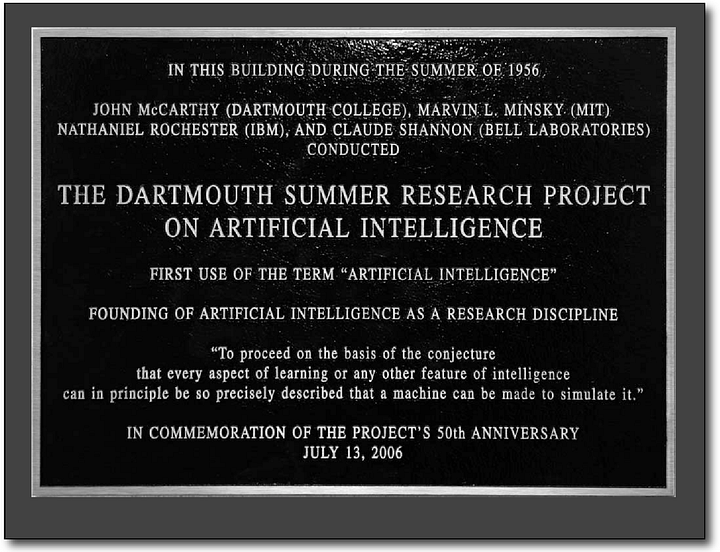
\includegraphics[width=0.98\textwidth]{./images/misc/dartmouth_commemorative_plaque.png}\\
            { \scriptsize 
            \vspace{0.1cm}
            Dartmouth Hall Commemorative Plaque..\\
            \color{col:attribution} 
            Photo by Joe Mehling, taken from \cite{Veisdal:2019dartmouth}.\\}
            \end{center}
        \end{column}
        \begin{column}{0.70\textwidth}
        \end{column}
    \end{columns}

\end{frame}


\subsection{Symbolic AI (1956-1974)}
\subsection{First AI winter (1974-1980)}
\subsection{Boom (1980-1987)}
\subsection{Bust: Second AI winter (1987-1993)}
\subsection{AI (1993-2011)}
\subsection{Deep learning, big data and AI (2011-present)}


%
%
%


\begin{frame}[t]{Effect of increased data}

    \vspace{-0.3cm}
    \begin{columns}
        \begin{column}{0.50\textwidth}
         \begin{center}
          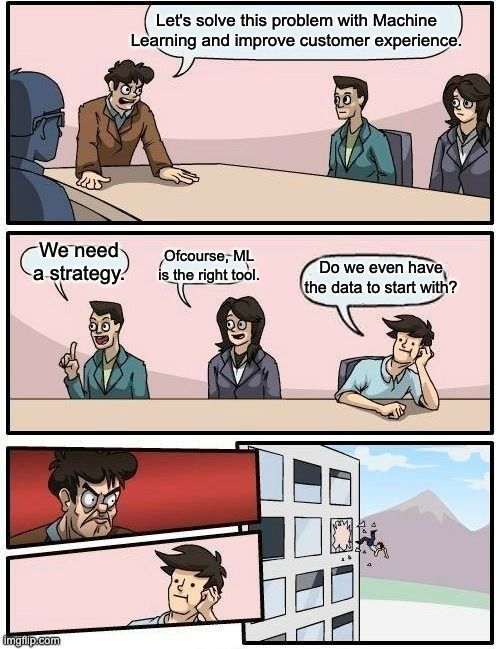
\includegraphics[width=0.99\textwidth]{./images/memes/do_we_even_have_data.png}
        \end{center}  
        \end{column}
        \begin{column}{0.50\textwidth}
            In     \gls{ml}
            {\scriptsize 
            \color{col:attribution} 
            %Image taken from \href{https://twitter.com/kdnuggets}{https://twitter.com/kdnuggets}
            }
        \end{column}
    \end{columns}

\end{frame}


\begin{frame}[t]{Effect of increased data}

    \begin{columns}
        \begin{column}{0.50\textwidth}
         \begin{center}
          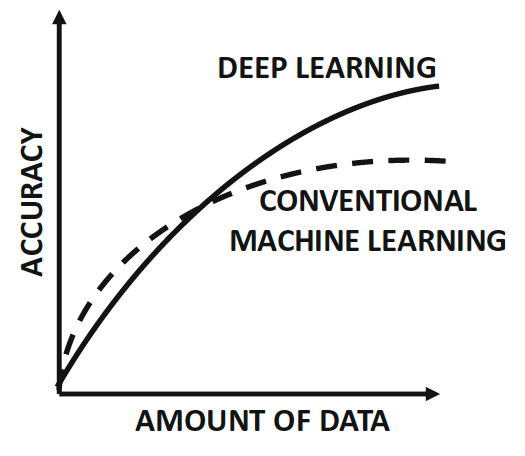
\includegraphics[width=0.95\textwidth]{./images/dl_intro/accuracy_vs_amount_of_data_1.png}\\
          {\scriptsize \color{col:attribution} 
          Image reproduced from p.54 of \cite{Aggarwal:2018SpringerDL}}\\
         \end{center}
        \end{column}
        \begin{column}{0.50\textwidth}
        \end{column}
    \end{columns}

\end{frame}

%
%
%

\begin{frame}[t,allowframebreaks]{Increasing neural network size - }

    % Intro

    % Number of connections in various artificial neural nets as a function of time
    % and comparison with biological brains

    The human brain has $\sim$100 billion neurons and $\sim$100 trillion synapses!

    \begin{center}
        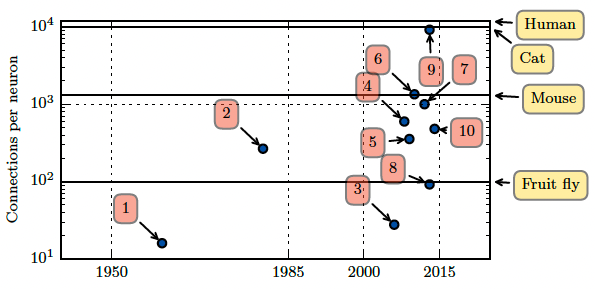
\includegraphics[width=0.95\textwidth]
          {./images/dl_intro/nnet_size_connections_vs_time_01.png}\\
        {\scriptsize \color{col:attribution} 
        Reproduced from p.22 of \cite{Goodfellow:2017DL}}\\
    \end{center}

    \framebreak

    % Number of neurons in various artificial neural nets as a function of time
    % and comparison with biological brains

    \begin{center}
        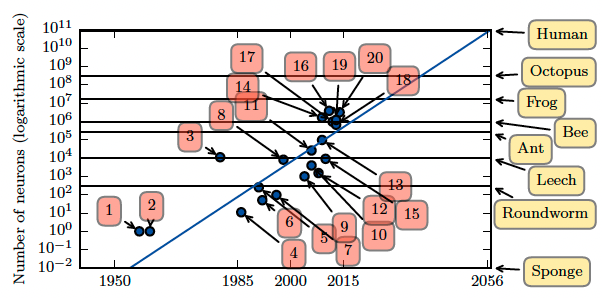
\includegraphics[width=0.95\textwidth]
           {./images/dl_intro/nnet_size_neurons_vs_time_01.png}\\
        {\scriptsize \color{col:attribution} 
        Reproduced from p.23 of \cite{Goodfellow:2017DL}}\\
    \end{center}
       {\tiny
       1. Perceptron (1958) \cite{Rosenblatt:1958p},
       2. Adaptive linear element (1960) \cite{Widrow:1960as},
       3. Neocognitron (1980) \cite{Fukushima:1980nc},
       4. Early back-propagation network (1986) \cite{Rumelhart:1986erp},
       5. Recurrent neural network for speech recognition (1991) \cite{Robinson:1991rerp},
       6. Multilayer perceptron for speech recognition (1991) \cite{Bengio:1991pma},
       7. Mean field sigmoid belief network (1996) \cite{Saul:1996mf},
       8. LeNet-5 (1998) \cite{LeCun:1998ln5},

       9. Echo state network (2004) (Jaeger and Haas, 2004)
       10. Deep belief network (2006) (Hinton et al., 2006)
       11. GPU-accelerated convolutional network (2006) (Chellapilla et al., 2006)
       12. Deep Boltzmann machine (2009) (Salakhutdinov and Hinton, 2009a)
       13. GPU-accelerated deep belief network (2009) (Raina et al., 2009)
       14. Unsupervised convolutional network (2009) (Jarrett et al., 2009)
       15. GPU-accelerated multilayer perceptron (2010) (Ciresan et al., 2010)
       16. OMP-1 network (2011) (Coates and Ng, 2011)
       
       17. Distributed autoencoder (2012) \cite{Le:2012daut}
       18. Multi-GPU convolutional network (2012) \cite{Krizhevsky:2012img},
       19. COTS HPC unsupervised convolutional network (2013) \cite{Coates:2013cots},       
       20. GoogLeNet (2014) \cite{Szegedy:2014gnet}\\
       }

    \framebreak

    % Information from recent well-known artificial neural networks

    \begin{itemize}
        \item GPT-2 had 1.5 billion parameters and around 50 billion neurons
        \item GPT-3 is estimated to have around 60-80 billion neurons
        \item GPT-4 is estimated to have around 60-80 billion neurons
    \end{itemize}

\end{frame}



\section{Different learning paradigms: Supervised, unsupervised and reinforcement learning}

\section{Artificial intelligence, machine learning and deep learning}

\section{Machine learning algorithms}

\begin{frame}[t]{Learning algorithms}


    A \index{ML}\gls{ml} algorithm 
    is one {\bf that is able to learn from data}.\\
    \vspace{0.2cm}

    An algorithm is said to learn from experience $E$ with respect to
    some class of tasks $T$ and performance metric $P$, 
    {\bf if its performance, as measured by $P$, at tasks in $T$,
    improves with experience $E$.}\\ 
    \vspace{0.2cm}

    Clearly, this can encompass a huge variety of examples\\

\end{frame}

\subsection{Machine learning tasks}


\begin{frame}[t]{Machine Learning tasks}

    Several tasks that can be solved by 
    \index{ML}\gls{ml} are listed below 
    (\cite{Goodfellow:2017MITDL}, Sec. 5.1.1):\\
    \vspace{0.2cm}
    \begin{itemize}
        \item
        \index{classification}\Gls{classification}.\\
        \vspace{0.1cm}
        \item
        \index{classification}\Gls{classification} with missing inputs.\\
        \vspace{0.1cm}
        \item
        \index{regression}\Gls{regression}.\\
        \vspace{0.1cm}
        \item
        \index{anomaly detection}\Gls{anomaly detection}
        (or \index{outlier detection}\gls{outlier detection}).\\
        \vspace{0.1cm}
        \item
        \index{structured output}\Gls{structured output}
        (or \index{structured prediction}\gls{structured prediction}).\\
        \vspace{0.1cm}
        \begin{itemize}
            \item
            Includes, as special categories,
            \index{transcription}\gls{transcription}
            and
            machine \index{translation}\gls{translation}.\\
            \vspace{0.1cm}
        \end{itemize}
        \item
        \index{synthesis and sampling}\Gls{synthesis and sampling}.\\
        \vspace{0.1cm}
        \item
        \index{denoising}\Gls{denoising}.\\
        \vspace{0.1cm}
        \item
        \index{density estimation}\Gls{density estimation}.\\
        \vspace{0.1cm}
        \item
        \index{dimensionality reduction}\Gls{dimensionality reduction}.\\
    \end{itemize}

    % \framebreak

    % %
    % %

    % \begin{itemize}
    %     \item
    %     {\bf \index{classification}\Gls{classification}} \\
    %     \vspace{0.1cm}
    %     \begin{itemize}
    %         {
    %             \item
    %             In this task, the \index{ML}\gls{ml} model 
    %             is asked to find in {\bf which of $k$ categories 
    %             some $n$-dimensional input belongs to}.
    %             \begin{itemize}
    %                 {\scriptsize
    %                 \item        
    %                 The model {\bf discovers a function 
    %                 $f: \mathbb{R}^n \rightarrow \{1,\dots,k\}$}
    %                 that assigns the category $y = f(\vect{x})$ 
    %                 of the input $\vect{x} \in \mathbb{R}^n$.\\
    %                 }
    %             \end{itemize}
    %             \vspace{0.1cm}
    %             \item
    %             Simple variants of this task include
    %             \index{probabilistic classification}\gls{probabilistic classification}.
    %             \begin{itemize}
    %                 {\scriptsize
    %                 \item        
    %                 The model discovers a 
    %                 function $f: \mathbb{R}^n \rightarrow [0,1]^k$
    %                 that outputs a {\bf probability distribution 
    %                 over the $k$ categories}.\\
    %                 }
    %             \end{itemize}
    %         }
    %     \end{itemize}
    %     \vspace{0.1cm}
    %     \item
    %     {\bf \index{classification}\Gls{classification} with missing inputs} \\
    %     \vspace{0.1cm}
    %     \begin{itemize}
    %         {
    %             \item The \gls{ml} model is not guaranteed 
    %             to have the full input vector $\vect{x} \in \mathbb{R}^n$.\\
    %             \begin{itemize}
    %                 {\scriptsize
    %                 \item        
    %                 The model discovers {\bf a set of functions} 
    %                 $f: \mathbb{R}^n \rightarrow \{1,\dots,k\}$, 
    %                 with $m \le n$, so the $\vect{x}$ can be classified
    %                 regardless of which subset of its elements missing!\\
    %                 }
    %             \end{itemize}
    %             \vspace{0.1cm}
    %             This task {\bf arises frequently in many real-world applications}.\\
    %             \begin{itemize}
    %                 {\scriptsize
    %                     \item
    %                     E.g in medical diagnosis where filling-in the 
    %                     full vector $\vect{x}$ may be invasive or expensive, 
    %                     or where failures in hardware or software 
    %                     lead to partial loss of data.\\
    %                 }
    %             \end{itemize}
    %         }
    %     \end{itemize}
    
    % \end{itemize}

    % \framebreak

    % %
    % %
    
    % \begin{itemize}
    %     \item
    %     {\bf \index{regression}\Gls{regression}} \\
    %     \vspace{0.1cm}
    %     \begin{itemize}
    %         {
    %             \item
    %             In this type of task, the \index{ML}\gls{ml} model 
    %             is asked to {\bf predict a numerical value given 
    %             some $n$-dimensional input}.
    %             \begin{itemize}
    %                 {\scriptsize
    %                 \item        
    %                 The model {\bf discovers a function 
    %                 $f: \mathbb{R}^n \rightarrow \mathbb{R}$
    %                 that calculates the value $y = f(\vect{x})$ 
    %                 for the input $\vect{x} \in \mathbb{R}^n$}.\\
    %                 }
    %             \end{itemize}
    %             \vspace{0.1cm}
    %             \item
    %             The task has similarities with 
    %             \index{classification}\gls{classification}. 
    %             \Gls{regression} tasks can be formulated 
    %             as \gls{classification} ones, and vice versa.\\
    %             \vspace{0.1cm}
    %             \item
    %             Example applications include 
    %             predicting tomorrow's stock prices, 
    %             or the average global temperature in the next century.
    %         }
    %     \end{itemize}
    %     \vspace{0.1cm}

    %     \item
    %     {\bf \index{anomaly detection}\Gls{anomaly detection}} 
    %     (or \index{outlier detection}\gls{outlier detection})\\
    %     \vspace{0.1cm}
    %     \begin{itemize}
    %         {
    %             \item
    %             In this \gls{ml} task, a model processes a set of data examples
    %             and {\bf flags some of them as being unusual}.
    %             \vspace{0.1cm}
    %             \item
    %             Example applications include, amongst many others,
    %             video surveillance and the detection of 
    %             credit card fraud, 
    %             intrusion, or 
    %             irregularities in the operation of complex machinery.
    %         }
    %     \end{itemize}

    % \end{itemize}

    % \framebreak

    % %
    % %
    
    % \begin{itemize}

    %     \item
    %     {\bf \index{structured output}\Gls{structured output}} 
    %     (or \index{structured prediction}\gls{structured prediction})\\
    %     \vspace{0.1cm}
    %     \begin{itemize}
    %         {
    %             \item
    %             In this type of task, a model outputs
    %             a vector of data, with important relationships between 
    %             the different elements of the vector.\\
    %             \vspace{0.1cm}
    %             \item 
    %             \Gls{structured output} is an umbrella term that includes,
    %             amongst other tasks, 
    %             \gls{transcription} 
    %             and machine \gls{translation} (see below).                 
    %         }
    %     \end{itemize}

    %     \item
    %     {\bf \index{transcription}\Gls{transcription}} \\
    %     \vspace{0.1cm}
    %     \begin{itemize}
    %         {
    %             \item
    %             Observing a relatively unstructured 
    %             representation of some type of data and converting it into
    %             discrete textual form.\\
    %             \vspace{0.1cm}
    %             \item 
    %             Common \gls{transcription} examples are 
    %             \index{Speech-to-Text}\Gls{speech-to-text} models
    %             and \index{OCR}\gls{ocr}.
    %         }
    %     \end{itemize}

    %     \item
    %     {\bf \index{translation}\Gls{translation}} \\
    %     \vspace{0.1cm}
    %     \begin{itemize}
    %         {
    %             \item
    %             Automatic conversion of a sequence of textual data in one 
    %             language is to another language.\\
    %         }
    %     \end{itemize}

    % \end{itemize}

    % \framebreak

    % %
    % %

    % \begin{itemize}

    %     \item
    %     {\bf \index{synthesis and sampling}\Gls{synthesis and sampling}} \\
    %     \vspace{0.1cm}
    %     \begin{itemize}
    %         {
    %             \item
    %             A task involving the automatic generation of examples 
    %             that are similar to those in the 
    %             \index{training set}\gls{training set}
    %             presented to the \index{ML}\gls{ml} model.\\
    %             \vspace{0.1cm}
    %             \item
    %             Examples include \\
    %         }
    %     \end{itemize}
    %     \vspace{0.1cm}

    %     \item
    %     {\bf \index{denoising}\Gls{denoising}} \\
    %     \vspace{0.1cm}
    %     \begin{itemize}
    %         {
    %             \item
    %             Presented with a corrupted data example 
    %             $\vect{\tilde{x}} \in \mathbb{R}^n$,
    %             produced by some unknown corrupting process acting 
    %             $\vect{x} \in \mathbb{R}^n$, 
    %             the \index{ML}\gls{ml} model is asked to predict
    %             the original example $\vect{x}$ or the
    %             conditional probability $p(\vect{x}|\vect{\tilde{x}})$. \\
    %             \vspace{0.1cm}
    %             \item
    %             Examples include \\
    %         }
    %     \end{itemize}
    %     \vspace{0.1cm}

    %     \item
    %     {\bf \index{density estimation}\Gls{density estimation}} \\
    %     \vspace{0.1cm}
    %     \begin{itemize}
    %         {
    %             \item
    %             In this task, a \gls{ml} model is asked to
    %             learn a function $p_{model}: \mathbb{R}^n \rightarrow \mathbb{R}$,
    %             where $p_{model}(\vect{x})$ can be interpreted as a 
    %             \index{probability density function}\gls{probability density function} 
    %             (\index{probability mass function}\gls{probability mass function}) 
    %             if $\vect{x}$ is continuous (discrete).\\
    %             \vspace{0.1cm}
    %             \item
    %             Examples include \\
    %         }
    %     \end{itemize}

    % \end{itemize}

    % \framebreak

    % %
    % %

    % \begin{itemize}

    %     \item
    %     {\bf \index{missing data imputation}\Gls{missing data imputation}} \\
    %     \vspace{0.1cm}
    %     \begin{itemize}
    %         {
    %             \item
    %             In this \gls{ml} task, a model is presented with a data example
    %             $\vect{x} \in \mathbb{R}^n$ missing values for a number of entries,
    %             and it is asked to predict the missing values.\\
    %             \vspace{0.1cm}
    %             \item
    %             Examples include \\
    %         }
    %     \end{itemize}

    % \end{itemize}

\end{frame}


\subsubsection{Classification}


\begin{frame}[t,allowframebreaks]{
    Machine Learning task: Classification - }

    \begin{itemize}
        {
            \item
            In \index{classification}\gls{classification} tasks, 
            the \index{ML}\gls{ml} model 
            is asked to find in {\bf which of $k$ categories 
            some $n$-dimensional input belongs to}.\\
            \vspace{0.1cm}
            \begin{itemize}
                {\small
                \item        
                The model {\bf discovers a function 
                $f: \mathbb{R}^n \rightarrow \{1,\dots,k\}$}
                that assigns the category $y = f(\vect{x})$ 
                of the input $\vect{x} \in \mathbb{R}^n$.\\
                }
            \end{itemize}
            \vspace{0.1cm}
            \item
            Simple variants of this task include
            \index{probabilistic classification}\gls{probabilistic classification}.\\
            \vspace{0.1cm}
            \begin{itemize}
                {\small
                \item        
                The model discovers a 
                function $f: \mathbb{R}^n \rightarrow [0,1]^k$
                that outputs a {\bf probability distribution 
                over the $k$ categories}.\\
                }
            \end{itemize}
        }
    \end{itemize}

\end{frame}
\subsubsection{Classification with missing inputs}

\begin{frame}[t,allowframebreaks]{
    Machine Learning task: Classification (missing inputs) - }

    \index{classification}\Gls{classification} with missing inputs
    
    \begin{itemize}
        {
            \item The \gls{ml} model is not guaranteed 
            to have the full input vector $\vect{x} \in \mathbb{R}^n$.\\
            \begin{itemize}
                {\scriptsize
                \item        
                The model discovers {\bf a set of functions} 
                $f: \mathbb{R}^n \rightarrow \{1,\dots,k\}$, 
                with $m \le n$, so the $\vect{x}$ can be classified
                regardless of which subset of its elements missing!\\
                }
            \end{itemize}
            \vspace{0.1cm}
            This task {\bf arises frequently in many real-world applications}.\\
            \begin{itemize}
                {\scriptsize
                    \item
                    E.g in medical diagnosis where filling-in the 
                    full vector $\vect{x}$ may be invasive or expensive, 
                    or where failures in hardware or software 
                    lead to partial loss of data.\\
                }
            \end{itemize}
        }
    \end{itemize}

\end{frame}
\subsubsection{Regression}


\begin{frame}[t,allowframebreaks]{
    Machine Learning task: Regression - }

    {\bf \index{regression}\Gls{regression}} \\
    \vspace{0.1cm}
    \begin{itemize}
        {
            \item
            In this type of task, the \index{ML}\gls{ml} model 
            is asked to {\bf predict a numerical value given 
            some $n$-dimensional input}.
            \begin{itemize}
                {\scriptsize
                \item        
                The model {\bf discovers a function 
                $f: \mathbb{R}^n \rightarrow \mathbb{R}$
                that calculates the value $y = f(\vect{x})$ 
                for the input $\vect{x} \in \mathbb{R}^n$}.\\
                }
            \end{itemize}
            \vspace{0.1cm}
            \item
            The task has similarities with 
            \index{classification}\gls{classification}. 
            \Gls{regression} tasks can be formulated 
            as \gls{classification} ones, and vice versa.\\
            \vspace{0.1cm}
            \item
            Example applications include 
            predicting tomorrow's stock prices, 
            or the average global temperature in the next century.
        }
    \end{itemize}

\end{frame}
\subsubsection{Anomaly detection (outliner detection)}

\begin{frame}[t,allowframebreaks]{
    Machine Learning task: Anomaly detection - }

    {\bf \index{anomaly detection}\Gls{anomaly detection}} 
    (or \index{outlier detection}\gls{outlier detection})\\
    \vspace{0.1cm}
    \begin{itemize}
        {
            \item
            In this \gls{ml} task, a model processes a set of data examples
            and {\bf flags some of them as being unusual}.
            \vspace{0.1cm}
            \item
            Example applications include, amongst many others,
            video surveillance and the detection of 
            credit card fraud, 
            intrusion, or 
            irregularities in the operation of complex machinery.
        }
    \end{itemize}

\end{frame}
\subsubsection{Structured output (structured prediction)}

\begin{frame}[t,allowframebreaks]{
    Machine Learning task: Structured output - }


    {\bf \index{structured output}\Gls{structured output}} 
    (or \index{structured prediction}\gls{structured prediction})\\
    \vspace{0.1cm}
    \begin{itemize}
        {
            \item
            In this type of task, a model outputs
            a vector of data, with important relationships between 
            the different elements of the vector.\\
            \vspace{0.1cm}
            \item 
            \Gls{structured output} is an umbrella term that includes,
            amongst other tasks, 
            \gls{transcription} 
            and machine \gls{translation} (see below).                 
        }
    \end{itemize}

    {\bf \index{transcription}\Gls{transcription}} \\
    \vspace{0.1cm}
    \begin{itemize}
        {
            \item
            Observing a relatively unstructured 
            representation of some type of data and converting it into
            discrete textual form.\\
            \vspace{0.1cm}
            \item 
            Common \gls{transcription} examples are 
            \index{Speech-to-Text}\Gls{speech-to-text} models
            and \index{OCR}\gls{ocr}.
        }
    \end{itemize}

    {\bf \index{translation}\Gls{translation}} \\
    \vspace{0.1cm}
    \begin{itemize}
        {
            \item
            Automatic conversion of a sequence of textual data in one 
            language is to another language.\\
        }
    \end{itemize}

\end{frame}
\subsubsection{Synthesis and sampling}


\begin{frame}[t,allowframebreaks]{
    Machine Learning task: Synthesis and sampling - }

    {\bf \index{synthesis and sampling}\Gls{synthesis and sampling}} \\
    \vspace{0.1cm}
    \begin{itemize}
        {
            \item
            A task involving the automatic generation of examples 
            that are similar to those in the 
            \index{training set}\gls{training set}
            presented to the \index{ML}\gls{ml} model.\\
            \vspace{0.1cm}
            \item
            Examples include \\
        }
    \end{itemize}

\end{frame}
\subsubsection{Denoising}

\begin{frame}[t,allowframebreaks]{
    Machine Learning task: Denoising - }

    {\bf \index{denoising}\Gls{denoising}} \\
    \vspace{0.1cm}
    \begin{itemize}
        {
            \item
            Presented with a corrupted data example 
            $\vect{\tilde{x}} \in \mathbb{R}^n$,
            produced by some unknown corrupting process acting 
            $\vect{x} \in \mathbb{R}^n$, 
            the \index{ML}\gls{ml} model is asked to predict
            the original example $\vect{x}$ or the
            conditional probability $p(\vect{x}|\vect{\tilde{x}})$. \\
            \vspace{0.1cm}
            \item
            Examples include \\
        }
    \end{itemize}

\end{frame}
\subsubsection{Density estimation}

\begin{frame}[t,allowframebreaks]{
    Machine Learning task: Density estimation - }

    {\bf \index{density estimation}\Gls{density estimation}} \\
    \vspace{0.1cm}
    \begin{itemize}
        {
            \item
            In this task, a \gls{ml} model is asked to
            learn a function $p_{model}: \mathbb{R}^n \rightarrow \mathbb{R}$,
            where $p_{model}(\vect{x})$ can be interpreted as a 
            \index{probability density function}\gls{probability density function} 
            (\index{probability mass function}\gls{probability mass function}) 
            if $\vect{x}$ is continuous (discrete).\\
            \vspace{0.1cm}
            \item
            Examples include \\
        }
    \end{itemize}

\end{frame}
\subsubsection{Missing data imputation}

\begin{frame}[t,allowframebreaks]{
    Machine Learning task: Imputation of missing data - }

    {\bf \index{missing data imputation}\Gls{missing data imputation}} \\
    \vspace{0.1cm}
    \begin{itemize}
        {
            \item
            In this \gls{ml} task, a model is presented with a data example
            $\vect{x} \in \mathbb{R}^n$ missing values for a number of entries,
            and it is asked to predict the missing values.\\
            \vspace{0.1cm}
            \item
            Examples include \\
        }
    \end{itemize}


\end{frame}

\subsection{Machine learning performance metrics}
\input{parts/introduction/learning_algorithms_performance_metrics.tex}

\subsection{Machine learning experience}
%
%
%

\begin{frame}[t]{Learning by experience}

    A \index{ML}\gls{ml} algorithm can {\bf learn from experience}.\\
    \vspace{0.2cm}
    Often, this should be understood as {\bf experiencing a dataset}.
    \begin{itemize}
        \item 
        \small
        A dataset is a collection of several data examples or data ``points".\\
    \end{itemize}
    \vspace{0.1cm}
    Depending on the type of experience,
    we distinguish between:\\
    \vspace{0.1cm}
    \begin{itemize}
        \item 
        {\bf \index{supervised learning}\gls{supervised learning}}, 
        where the data examples include {\bf labels} to teach the algorithm
        how to make correct decisions,
        and\\
        \vspace{0.1cm}
        \item 
        {\bf \index{unsupervised learning}\gls{unsupervised learning}},
        where the algorithm is trying to deduce relationships and patterns
        within a set of {\bf unlabelled} examples.\\
    \end{itemize}
    \vspace{0.1cm}
    The above {\bf distinction is often blurred}.\\

    \vspace{0.2cm}

    Some \gls{ml} algorithms do not experience a fixed dataset:
    Instead, they are allowed to {\bf interact with the environment}.
    \begin{itemize}
        \item 
        The term
        {\bf \index{reinforcement learning}\gls{reinforcement learning}}
        describes this learning paradigm.\\
    \end{itemize}

\end{frame}


\subsubsection{Supervised learning}
%
%
%

\begin{frame}[t,allowframebreaks]{
    Learning paradigm: Supervised learning - }

\index{supervised learning}\gls{supervised learning}

\end{frame}
\subsubsection{Unsupervised learning}
%
%
%

\begin{frame}[t,allowframebreaks]{
    Learning paradigm: Unsupervised learning - }

    On the other hand, 
    in \index{unsupervised learning}\gls{unsupervised learning},
    an algorithm experiences a dataset where the is 
    {\bf no label associated to each example}.\\
    \vspace{0.2cm}

    Undirected, the algorithm 
    {\bf discovers useful properties of the dataset}.\\
    \vspace{0.2cm}

    In this learning paradigm, by observing many 
    examples ${\vect{x}}$, the \gls{ml} model is attempting to
    {\bf learn the data generating probability 
    distribution $p(\vect{x})$} 
    \begin{itemize}
      \item or, simply, to learn certain interesting properties of that distribution.\\
    \end{itemize}
    

\end{frame}
\subsubsection{Reinforcement learning}
%
%
%

\begin{frame}[t,allowframebreaks]{
    Learning paradigm: Reinforcement learning - }

    \index{reinforcement learning}\gls{reinforcement learning}

\end{frame}
\subsubsection{Blurring the boundaries of learning paradigms}
%
%
%

\begin{frame}[t,allowframebreaks]{
    Learning paradigm blurring - }

    The previously used terms of
    \index{supervised learning}\gls{supervised learning},
    \index{unsupervised learning}\gls{unsupervised learning}, and
    \index{reinforcement learning}\gls{reinforcement learning}
    are {\bf not formally defined.}\\
    \vspace{0.2cm}

    Indeed the {\bf boundaries are blurred}, especially between
    \gls{supervised learning} and \gls{unsupervised learning},
    and many technologies can perform both tasks.\\
    \vspace{0.2cm}

    Recall that in \gls{supervised learning} the algorithm learns
    the conditional probability $p(\vect{y}|\vect{x})$, whereas in
    \gls{unsupervised learning} it learns the 
    probability distribution  $p(\vect{x})$.\\

    \begin{equation}
        p(\vect{x}) = p(x_1 | x_2, \dots, x_n) p(x_2, \dots, x_n)
    \end{equation}

    \begin{equation}
        p(\vect{x}) = \prod_{i=1}^{n} p(x_i | x_2, \dots, x_{i-1})
    \end{equation}

\end{frame}

\section{A simple practical example: Linear regression}

%
%
%

\begin{frame}[t]{Example: Linear regression}

    To clarify the previous ideas, 
    we will study a concrete example
    of a \index{ML}\gls{ml} algorithm: 
    \index{linear regression}{\bf \gls{linear regression}}$^{1}$.\\
    \vspace{0.2cm}
    Although this is a very simple algorithm with limited capabilities,
    it is an instructive example.\\
    \vspace{0.2cm}

    As we discussed previously, 
    to define our \gls{ml} problem we need to define:\\
    \vspace{0.1cm}

    \begin{itemize}
        \item 
        the {\bf task} - 
        i.e. what do we want to learn,\\
        \vspace{0.1cm}
        \item 
        the {\bf experience} - 
        i.e. where are we going to learn from, and\\
        \vspace{0.1cm}
        \item 
        the {\bf performance metric} - 
        i.e. what learning performance measure are trying to optimise?\\
    \end{itemize}

    \vspace{0.2cm}
    \noindent\rule{4cm}{0.4pt}\\
    {\scriptsize
      $^{1}$ We will revisit \gls{linear regression}
      in subsequent lectures.\\
    }

\end{frame}

%
%
%

\begin{frame}[t]{Example: Linear regression / Task}

    {\bf \Gls{linear regression} solves a 
    \index{regression}\gls{regression} problem}.\\
    \vspace{0.2cm}

    Our goal is to build a system that 
    accepts as input a vector $\vect{x} \in \mathbb{R}^n$
    and predicts a scalar variable $y \in \mathbb{R}$ as output.\\
    \vspace{0.2cm}

    In \gls{linear regression}, the output is a 
    {\bf linear function}$^{1}$ of the input $\vect{x}$:
    \begin{equation}
        \hat{y} = \vect{w}^T \vect{x}
        \label{eq:intro_linear_regression_model}
    \end{equation}
    where $\vect{w} \in \mathbb{R}^n$ is a vector of model parameters 
    whose values need to be ``learned", and 
    the output $\hat{y}$ is the model prediction of $y$.\\
    \vspace{0.2cm}

    One can think of the parameters $\vect{w}$ as {\bf weights}
    that determine how each {\bf feature} 
    (element of input $\vect{x}$)
    affects the prediction.\\

    \vspace{0.2cm}
    \noindent\rule{4cm}{0.4pt}\\
    {\scriptsize      
      $^{1}$ In general, we could have written this as
      $\hat{y} = \vect{w}^T \vect{x} + b$, introducing a bias $b$.
      However, the same effect could be achieved with the linear model of 
      Eq.~\ref{eq:intro_linear_regression_model}, by expanding $\vect{x}$
      with the addition of a new feature whose value is always 1.\\
    }

\end{frame}

%
%
%

\begin{frame}[t,allowframebreaks]{
    Example: Linear regression / Performance metric - }

    The performance of the model can be described by the 
    \index{MSE}\gls{mse} over the 
    \index{test set}\gls{test set} $\mathbb{D}_{test}$:
    \begin{equation}
        MSE_{test} = 
          \mathbb{E}_{(\vect{x},y) \in \mathbb{D}_{test}}
           \sum_{(\vect{x},y) \in \mathbb{X}_{test}} 
                \Big(\vect{w}^T \vect{x} - y\Big)
        \label{eq:intro_linear_regression_model_mse_test}
    \end{equation}

\end{frame}


\section{Biologically inspired methods of computer learning}

\section{Basic architecture of neural networks}

\section{Fundamental concepts}
\begin{frame}[t,allowframebreaks]{Fundamental concepts - }

    \gls{relu}
\end{frame}


% From AI to DL
\begin{frame}{Connection between AI, ML and DL}

\index{AI}\index{artificial intelligence}\gls{ai} -
\gls{ai}
\gls{ml}
\gls{dl}

    \begin{center}
        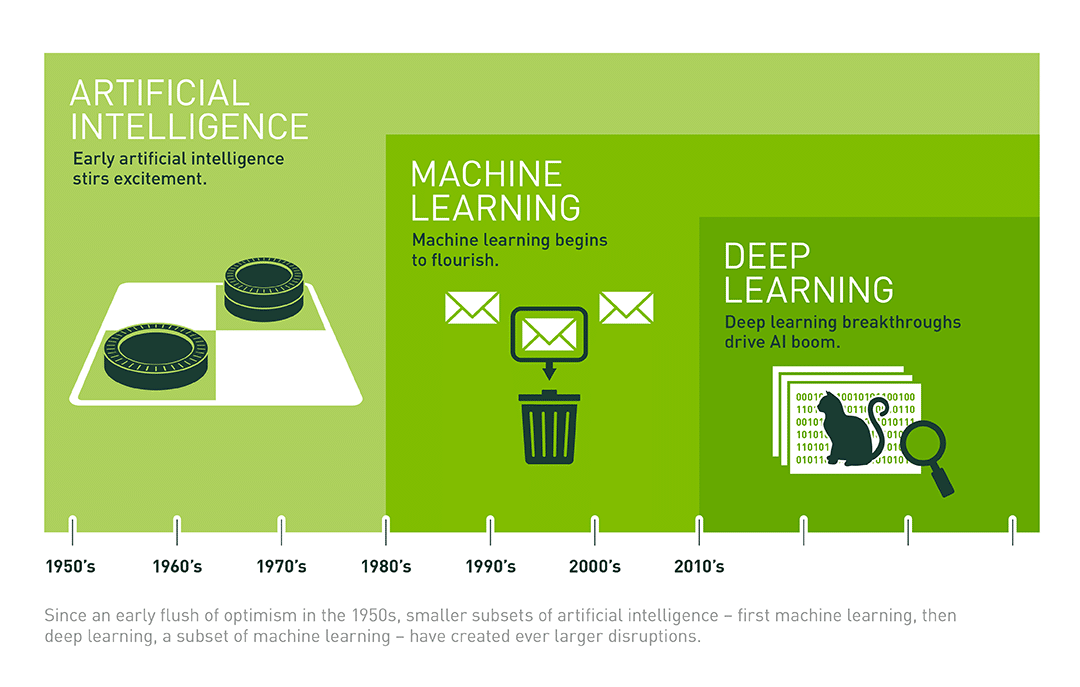
\includegraphics[width=0.90\textwidth]{./images/dl_intro/ai_ml_dl.png}\\
        {\scriptsize Image reproduced from \cite{NVidiaBlog:DifferenceBetweenAIMLDL}}\\
    \end{center}

\end{frame}
    


% Main points to remember
\renewcommand{\summarizedlecture}{1 }

%
%
%

\begin{frame}{Lecture \summarizedlecture - \lecturesummarytitle}


\end{frame}



% Suggested reading for this part
\section{Suggested reading}
%
%
%

\begin{frame}{Suggested reading for Part \thispart}

    {
        \small
        Essential reading on {\bf automatic differentiation}:
        \begin{itemize}
            \scriptsize
            \item Section 6.5 from the `Deep Learning' 
            textbook of Goodfellow, Bengio and Courville \cite{Goodfellow:2017MITDL}.
            \item Appendix B from the `Machine Learning Refined' 
            textbook of Watt, Borhani and Katsaggelos \cite{Watt:2016Cambridge}.
            \item `A review of automatic differentiation and its 
            efficient implementation' by Margossian \cite{Margossian:2019ad}
        \end{itemize}
        
        Also, you may want to browse:
        \begin{itemize}
            \scriptsize
            \item The collection of articles
             in the book `Automatic Differentiation: Applications, Theory, and Implementations'
             edited by B{\"u}cker, Corliss, Hovland, Naumann and Norris \cite{Bucker:2005ABo}
        \end{itemize}
    }
    

\end{frame}

% Optional material


